\documentclass[pmlr,twocolumn,10pt]{jmlr} % W&CP article

% REQUIRED: submission track. proceedings / findings / demo / perspective
\mlhtrack{proceedings}

\newif\iffinal
\finalfalse  % initial submission (review); switch to \finaltrue for camera-ready
% \finaltrue

\iffinal
    \ifmlhneedspmlr
      \jmlrvolume{XXX}
      \jmlryear{2026}
    \fi
    \ifmlhfindings \jmlrproceedings{}{ML4H 2026 - Findings Track}\fi
    \ifmlhdemo     \jmlrproceedings{}{ML4H 2026 - Demo Track}\fi
    \jmlrworkshop{Machine Learning for Health (ML4H) 2026}
\else
    \jmlrproceedings{}{Submitted to ML4H 2026: \mlhtrackname}
    \jmlrworkshop{Machine Learning for Health (ML4H) 2026}
\fi

\urlstyle{same}

\usepackage{booktabs}

% The lineno package is required for denoting line numbers for paper review.
\usepackage[switch]{lineno}

\title[Complexity vs Transportability in Ovarian Cancer Risk]{Model
Complexity Versus Transportability in Ovarian Cancer Risk Prediction: A
Cross-Cohort Benchmark with Decision Analysis}

% Anonymized author list during review
\author{Anonymous Author(s)}

\linenumbers % Activate line numbering

\begin{document}

\maketitle

\ifmlhdemo\else
\begin{abstract}
We test whether model complexity translates into transportable clinical
performance for preoperative ovarian-cancer risk stratification---the
serum-marker triage of the most lethal gynecologic malignancy---under
external distributional and structural shift. Eight
models---a one-parameter CA125 rule, two clinical formulas (ROMA, CPH-I),
an unbinned logistic regression, an integer scorecard with seven
whole-point weights, and three tree ensembles---were trained on a Chinese
cohort ($n=349$) and applied frozen to two external Asian cohorts (West
China, $n=380$; Japan, $n=177$). On the primary external validation cohort
(West China), the scorecard (AUROC 0.929) and the unbinned regression
(0.936) were statistically indistinguishable, and each exceeded the
remaining models (ROMA, CPH-I, and the tree ensembles); pooled across both
cohorts, the scorecard beat ROMA ($+0.043$, $p=0.006$) and all ensembles
($+0.046$ to $+0.054$, $p\le0.002$). The published cutpoints
missed 82 of 188 cancers versus 47 for the scorecard's high-risk tier. A
simulation calibrated to the training data provides a plausible
mechanistic account in which \emph{concept drift}---structural change in
the marker-to-outcome mapping---produces the observed ranking. For
small-sample clinical ML, external validation and drift-aware simulation
distinguish what transfers from what merely fits.
\end{abstract}

\begin{keywords}
ovarian cancer; risk prediction; integer scorecard; external validation;
transportability; distribution shift; decision curve analysis
\end{keywords}
\fi

\ifmlhneedsstatements
\paragraph*{Data and Code Availability}
The three cohorts are public, de-identified datasets archived at Mendeley
Data (Chinese training cohort, \url{https://doi.org/10.17632/th7fztbrv9.11}),
figshare (West China, \url{https://doi.org/10.6084/m9.figshare.28831256}),
and Karger figshare (Japan, \url{https://doi.org/10.6084/m9.figshare.24235450}).
All analysis code, figure scripts, and benchmark outputs are available in
an anonymized code repository included as supplemental material with this
submission; the repository will be de-anonymized and made public at
\url{https://github.com/angelayaoo/Ovarian-Cancer-RiskSLIM} for the
camera-ready version. The repository includes a one-command pipeline
(\texttt{reproduce.sh}) that regenerates every table and figure from the
public cohorts, with pinned dependencies and all intermediate results
archived.

\paragraph*{Institutional Review Board (IRB)}
This is a secondary analysis of fully de-identified, publicly archived data;
no IRB approval is required in the originating jurisdictions, and the
originating studies obtained their own approvals in line with the
Declaration of Helsinki.
\fi

\section{Introduction}

Preoperative risk assessment decides which women with an ovarian mass are
referred to oncologic surgery, and it leans on two serum markers, CA125 and
HE4, combined into fixed formulas such as ROMA \citep{moore2011} and the
Copenhagen Index CPH-I \citep{karlsen2015}. Machine-learning models have
been proposed repeatedly for this task \citep{kawakami2019,lu2020}, usually
with strong internal performance and little external evidence. The broader
clinical-prediction literature has established three uncomfortable facts:
flexible models seldom beat well-regularized logistic regression on tabular
data, especially at the sample sizes of single hospitals
\citep{christodoulou2019,vanderploeg2014}; prediction models frequently fail
to transfer across settings \citep{roberts2021,wynants2020}; and
interpretable models belong in high-stakes medicine unless clearly worse
\citep{rudin2019,caruana2015}. What is missing is a systematic account of
\emph{when} complexity repays its cost, quantified across the dimensions
that matter for deployment: external discrimination, calibration, decision
consequences, robustness to measurement error, sample-size efficiency, and
structural drift.

Prior work shows flexible models often fail to beat logistic regression
\citep{christodoulou2019} and that prediction models degrade across
settings \citep{roberts2021,wynants2020}, but rarely quantifies
\emph{when} complexity pays: across what sample sizes, distribution shifts,
and structural changes. We address this gap with three public cohorts and a
pre-specified protocol. Contributions: (i) an eight-model benchmark with
selection and preprocessing frozen on the training cohort, so external
performance measures transportability; (ii) a decision-analytic
evaluation---operating points, weighted-harm analysis, decision
curves---showing where published cutpoints fail; (iii) a synthetic
simulation reproducing the empirical ranking under a structural-shift
account; and (iv) a factor decomposition quantifying each shift
component's contribution to the model gap. The protocol itself is the
transferable artifact for small-sample clinical ML.

\section{Related Work}

Reviews find no benefit of ML over logistic regression on tabular data
\citep{christodoulou2019}, and simulation studies show modern techniques
are ``data hungry'' \citep{vanderploeg2014,riley2020}. RiskSLIM learns
sparse integer scoring systems with certified optimality
\citep{ustun2016}; bedside-computable scores persist for this reason
\citep{caruana2015,rudin2019}. We combine paired bootstrap and DeLong tests, meta-analytic pooling,
calibration, and decision curves
\citep{delong1988,hanley1983,dersimonian1986,vancalster2019,vickers2006}
into one protocol, adding a drift-aware simulation.

\section{Setup}

\paragraph{Data.} Three public, de-identified Asian cohorts, archived at
Mendeley Data (Chinese; \url{https://doi.org/10.17632/th7fztbrv9.11}),
figshare (West China; \url{https://doi.org/10.6084/m9.figshare.28831256}),
and Karger figshare (Japan; \url{https://doi.org/10.6084/m9.figshare.24235450}).
The target population is women with a suspected ovarian mass and
preoperative CA125 and HE4 measured. Chinese training cohort: $n=349$ (171
ovarian cancers, 178 benign masses), 49 variables. West China: $n=380$ (188
cancers, 192 benign cysts); HE4 missing in 74\%. Japan: $n=177$ (27
cancers, 150 healthy women); age missing in 85\%. Because Japan contrasts cancers with healthy controls rather than
benign masses, it serves as an \emph{intentional} case-mix stress test
rather than a second triage validation: transportability claims should be
probed at the limits of their case mix, and a screening-like cohort is that
limit. Features: CA125 (U/mL), HE4 (pmol/L), age, menopausal status. External
missing values are replaced with per-feature training medians, frozen; no
statistic is computed on a validation cohort. The primary endpoint is the scorecard-versus-ROMA AUROC difference on
West China; all other analyses are secondary. The imputation strategy is
varied in the no-HE4 and complete-case sensitivity analyses (Results). Per-feature
Kolmogorov--Smirnov shifts versus the training distribution range
0.13--0.38 (West China, mean 0.22) and 0.43--0.60 (Japan, mean 0.50).

\paragraph{Models.} (1) \emph{Integer scorecard}: continuous features
rank-transformed, cut into three equal-frequency bins, fitted with
L2-regularized logistic regression, coefficients rescaled and rounded to
integers in $[-5,5]$: each coefficient is rescaled as
$w_i=\mathrm{round}(\beta_i \times 5 / \max_j|\beta_j|)$, with
$|\beta_i|<0.01$ set to zero. The configuration is
selected strictly internally by the one-standard-error rule over a
pre-specified 12-configuration grid (bins $\times$ regularization
strength), with all preprocessing refitted inside each training fold.
(2) \emph{Unbinned logistic regression} on standardized features.
(3--4) \emph{ROMA} \citep{moore2011} and \emph{CPH-I}
\citep{karlsen2015}, published formulas computed on the same median-imputed
raw features as every other model. (5) \emph{CA125 $\ge$ 35 U/mL rule}.
(6--8) \emph{XGBoost} \citep{chen2016} (100 trees, maximum depth 6,
learning rate 0.3), \emph{CatBoost} \citep{prokhorenkova2018} (1{,}000
iterations, depth 6, learning rate 0.03), and \emph{Random Forest}
\citep{breiman2001} (100 trees, no depth cap) at package defaults; a
27-configuration tuning grid and nested cross-validation are reported as
sensitivity analyses. Every model uses the same four features and the same
frozen preprocessing; models are trained once on the Chinese cohort and
applied unchanged everywhere else.

\paragraph{Evaluation protocol.} \emph{Discrimination}: AUROC per cohort;
pairwise comparisons by 2{,}000 patient-level paired bootstrap resamples
(two-sided empirical $p$-values); random-effects pooling across the two
external cohorts (DerSimonian--Laird \citep{dersimonian1986}) with $I^2$ as
the heterogeneity measure. \emph{Internal validity}: five-fold stratified
CV (StratifiedKFold, shuffle, seed 42) repeated 20 times; in-sample AUROC to quantify memorization; nested CV
(outer five-fold, inner five-fold over a 9-configuration grid per family)
for the tuned ensembles. \emph{Calibration}: Brier score; calibration-in-the-large, computed as
$\log(\bar{p}/(1-\bar{p})) - \log(\bar{y}/(1-\bar{y}))$; and LOWESS-smoothed
calibration curves (fraction 0.8, clipped to $[0,1]$). \emph{Decision
analysis}: sensitivity/specificity at published cutpoints; weighted-harm
analysis in which, for exchange-rate weights
$w\in\{1,2,5,10,20,50\}$ (harm of one missed cancer relative to one
unnecessary referral), the threshold minimizing
$H=w\cdot\text{missed}+\text{unnecessary}$ per 100 women is identified for
each model; decision curves with bootstrap bands \citep{vickers2006}.
\emph{Robustness}: Monte Carlo multiplicative noise on CA125/HE4 (0--30\%,
100 perturbations per level), additive and combined noise, 5\%
gross-error contamination, $\pm10\%$ cutpoint perturbation, and learning
curves retraining on $n=60$--$349$. \emph{Simulation}: a generative model
calibrated to the training data. Class-conditional biomarkers are sampled
as lognormal mixtures, $z_{k}\sim\mathcal{N}(m_{k}^{(y)},\,s_{k}^{(y)})$,
with class means and variances estimated per class from the Chinese
cohort's log-transformed CA125 and HE4 and raw age; the outcome follows a
Bernoulli model with frozen-standardized features,
\begin{equation}
\begin{split}
\eta(\mathbf{z}) &= -0.65 + 1.8\,z_{1} + 1.0\,z_{2} + 0.5\,z_{3}\\
& + (1-d)\bigl(1.6\,z_{1}z_{2} + 1.2\sin(1.7\,z_{1})\bigr),
\end{split}
\label{eq:eta}
\end{equation}
where $z_{1},z_{2},z_{3}$ are the standardized biomarkers and $d\in\{0,1\}$
is concept drift (under drift the interaction and nonlinear terms vanish
from the test-side outcome model). Factors: training size
$n\in\{100,200,400,800\}$; distribution shift implemented as shrinkage of
class-conditional means toward the pooled mean by $\delta\in\{0,0.5,1.0\}$
(plus variance inflation), so discrimination decreases monotonically in
$\delta$; multiplicative measurement noise on CA125/HE4,
$\sigma\in\{0,0.5\}$ (additive Gaussian on the log scale), applied only to
the test set; 20 replicates per cell; test $n=4{,}000$. Models are trained
on clean, stationary data and evaluated frozen on the shifted test set,
mirroring the real-cohort protocol. Implementation: Python 3.13,
scikit-learn 1.6, XGBoost 2.1, CatBoost 1.2, fixed seeds
(random\_state $=42$).

\section{Results}

We report external discrimination first, then internal validity and
calibration, decision consequences, robustness, and the simulation.

\subsection{External discrimination}

\paragraph{Discrimination on the primary external validation cohort.} On West China, the
scorecard (0.929, 95\% CI 0.902--0.955) and the unbinned logistic
regression (0.936, 0.908--0.961) were statistically indistinguishable
($p=0.48$). Both exceeded CPH-I (0.868), ROMA (0.886), and the tree ensembles
(0.879--0.887) (West column, \tableref{tab:auroc}); in the Japan column
CPH-I was highest (0.920). \figureref{fig:ladder} shows the per-model
values.

\begin{figure*}[htbp]
\floatconts
  {fig:ladder}
  {\caption{External AUROC on the West China cohort ($n=380$; 188 cancers,
   192 benign), with models ordered left to right by increasing complexity.
   Points are bootstrap means (2{,}000 resamples) with 95\% confidence
   intervals; values are printed above the points. Markers encode model
   family: circles = linear models, squares = published formulas,
   triangles = tree ensembles. ROMA = Risk of Ovarian Malignancy
   Algorithm; CPH-I = Copenhagen Index.}}
  {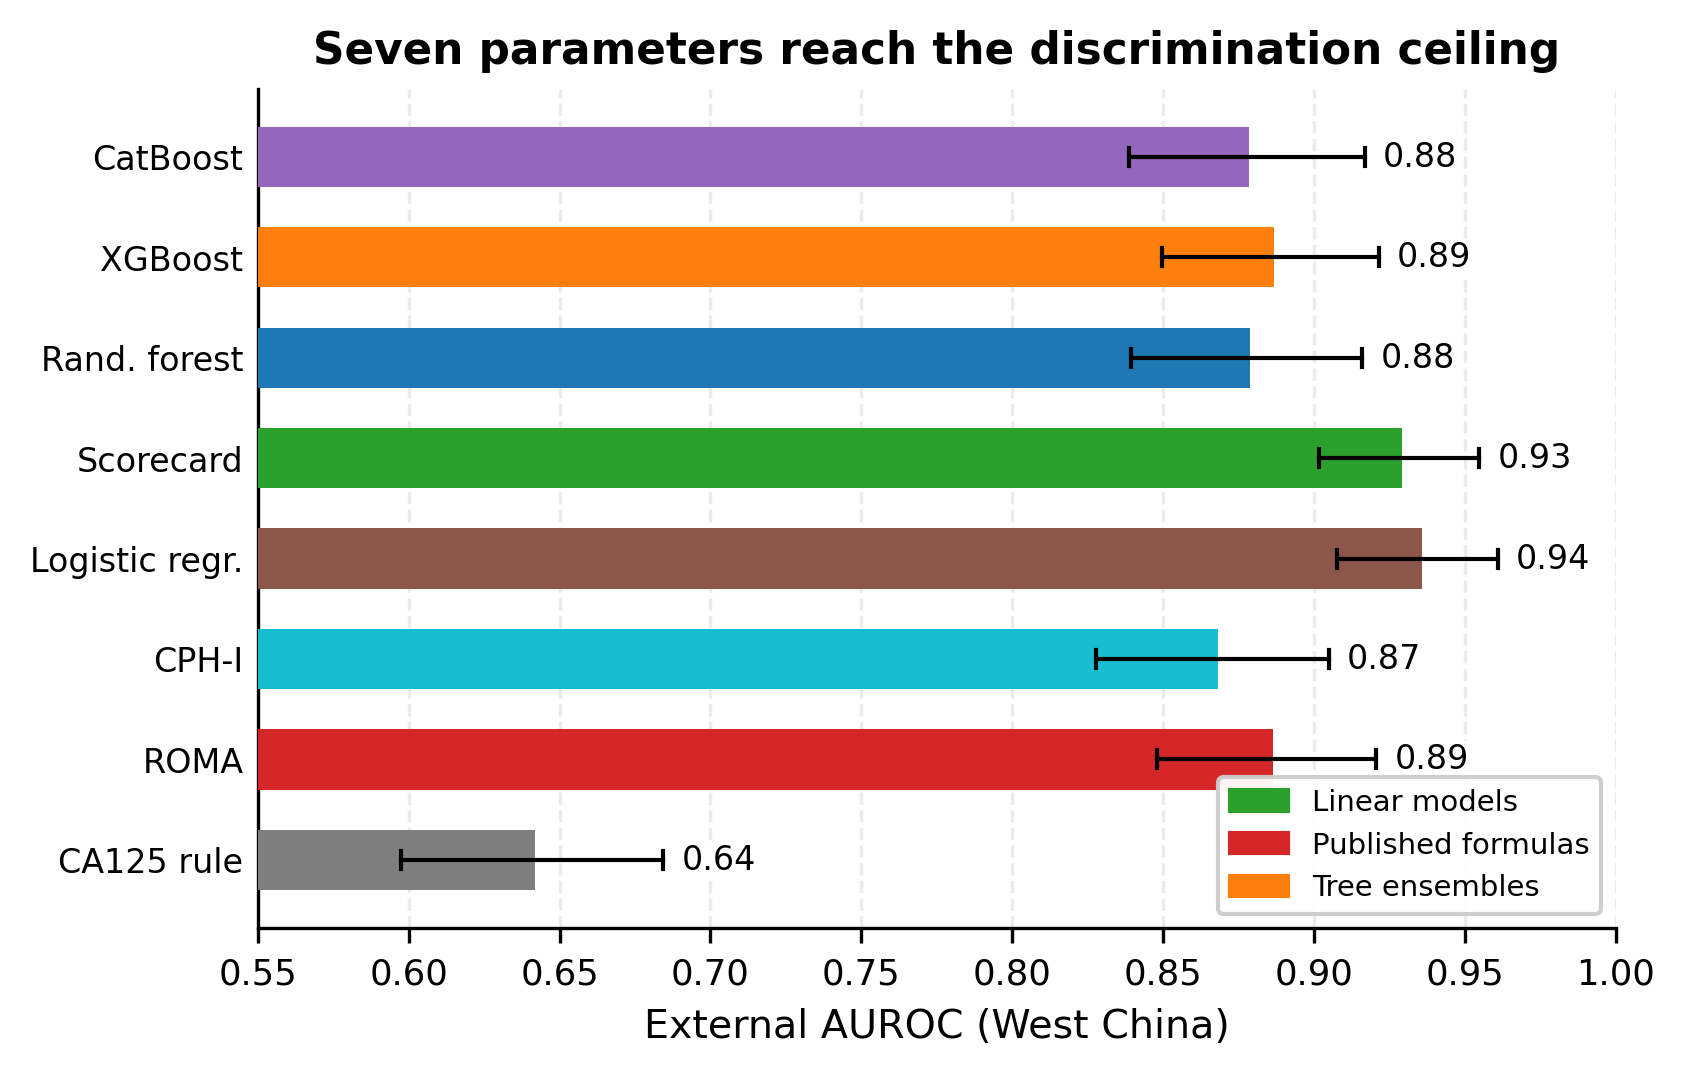
\includegraphics[width=0.66\textwidth]{figures/fig_ladder}}
\end{figure*}

\begin{table}[htbp]
\floatconts
  {tab:auroc}
  {\caption{AUROC by model and cohort at 0\% measurement noise. Train =
   five-fold cross-validated (CV) AUROC on the Chinese training cohort;
   West and Japan are bootstrap means on the external cohorts. Bold marks
   the cohort-wise best fitted model. $^{a}$ Published fixed formula
   (applied value, not fitted); ROMA = Risk of Ovarian Malignancy
   Algorithm; CPH-I = Copenhagen Index.}}
  {\setlength{\tabcolsep}{4pt}\begin{tabular}{lccc}
  \toprule
  Model & Train (CV) & West & Japan\\
  \midrule
  Scorecard & 0.906 & \textbf{0.929} & 0.843\\
  Logistic regr. & 0.894 & \textbf{0.936} & 0.804\\
  ROMA$^{a}$ & 0.912 & 0.886 & 0.797\\
  CPH-I$^{a}$ & 0.912 & 0.868 & \textbf{0.920}\\
  CA125 rule$^{a}$ & 0.727 & 0.642 & 0.781\\
  XGBoost & 0.882 & 0.887 & 0.734\\
  CatBoost & 0.900 & 0.879 & 0.749\\
  Random Forest & 0.895 & 0.879 & 0.792\\
  \bottomrule
  \end{tabular}}
\end{table}

\paragraph{Pooled external comparison.} Across both external cohorts
(\tableref{tab:meta}), the scorecard exceeded ROMA by $+0.043$ (95\% CI
0.013--0.074, $p=0.006$, $I^2=0$). It exceeded every tree ensemble by
$+0.046$ to $+0.054$ (all $p\le0.002$) and matched the unbinned regression
($-0.005$, $p=0.55$). $I^2$ was 0 for ROMA and for each tree ensemble.

\begin{table*}[htbp]
\floatconts
  {tab:meta}
  {\caption{Scorecard-minus-comparator AUROC differences. $\Delta$ West
   and $\Delta$ Japan are paired bootstrap differences (2{,}000
   patient-level resamples) on the West China cohort ($n=380$; 188
   cancers, 192 benign) and the Japanese stress-test cohort ($n=177$; 27
   cancers, 150 healthy women). Pooled = DerSimonian--Laird random-effects
   estimate across the two cohorts; CI = 95\% confidence interval;
   $I^2$ = heterogeneity statistic; $p$ = two-sided empirical p-value from
   the paired bootstrap. AUROC = area under the receiver operating
   characteristic curve.}}
  {\small\begin{tabular}{lrrrrrr}
  \toprule
  Comparator & $\Delta$ West & $\Delta$ Japan & Pooled & 95\% CI & $p$ & $I^2$\\
  \midrule
  Logistic regression & $-0.007$ & $+0.039$ & $-0.005$ & $-0.023$ to 0.012 & 0.554 & 0\%\\
  ROMA & $+0.043$ & $+0.046$ & $+0.043$ & 0.013 to 0.074 & 0.006 & 0\%\\
  CPH-I & $+0.061$ & $-0.076$ & $+0.005$ & $-0.127$ to 0.137 & 0.942 & 79\%\\
  CA125 rule & $+0.288$ & $+0.064$ & $+0.186$ & $-0.032$ to 0.404 & 0.094 & 89\%\\
  XGBoost & $+0.043$ & $+0.109$ & $+0.046$ & 0.017 to 0.074 & 0.002 & 0\%\\
  CatBoost & $+0.051$ & $+0.095$ & $+0.054$ & 0.024 to 0.084 & $<0.001$ & 0\%\\
  Random Forest & $+0.051$ & $+0.051$ & $+0.051$ & 0.022 to 0.080 & $<0.001$ & 0\%\\
  \bottomrule
  \end{tabular}}
\end{table*}

\paragraph{Heterogeneity.} The CPH-I comparison was the only heterogeneous
one ($I^2=79\%$): the difference was $+0.061$ in West China and $-0.076$ in
the Japanese cohort (27 cancers, 150 healthy women). In that cohort, 86\% of healthy women and 30\% of
cancer patients fell into the lowest training-calibrated bins of both
markers.

\paragraph{Internal validity.} Across 20 repeated five-fold CVs the
scorecard's mean internal AUROC was 0.906 (SD 0.003); the deployed
three-bin configuration was selected in 18 of 20 repeats. In-sample,
the ensembles fitted at 0.991--1.000 and fell by 0.094--0.117 under CV
(scorecard: 0.005); nested CV of tuned ensembles reached 0.885--0.903.

\subsection{Internal validity and calibration}

\paragraph{Calibration.} On West China (prevalence 49.5\%), Brier scores were 0.097
(recalibrated scorecard), 0.111 (unbinned regression), 0.128 (XGBoost),
0.209 (ROMA), and 0.259 (CPH-I). Calibration-in-the-large was $-0.95$
(ROMA) and $-1.42$ (CPH-I) \citep{rolfsen2020}.

\subsection{Decision consequences}

\paragraph{Decision consequences.} At its high-risk tier (score $\ge+1$)
the scorecard achieved 75.0\% sensitivity and 97.4\% specificity, missing
47 of 188 cancers with 5 false-positive referrals. At their published
cutpoints ROMA achieved 56.4\% sensitivity and 96.9\% specificity (82
cancers missed, 6 false positives); CPH-I achieved 74.5\% and 94.8\% (48
missed, 10 false positives). In the weighted-harm analysis
(\tableref{tab:harm}, \figureref{fig:cons}), the unbinned regression had
the lowest minimum harm at every exchange rate. The scorecard was within
2.4--7.6 harm points per 100 women of it and below ROMA at all rates
$\le10{:}1$. A second analysis applied the same within-cohort recalibration to the
published formulas: minimum harms were 12.1 (scorecard), 14.7 (ROMA), and
15.0 (CPH-I) at $w=1$, and 45.0, 45.8, and 49.5 at $w=10$; at $w=50$,
recalibrated ROMA (45.8) was below the scorecard (59.5). Decision curves with bootstrap bands placed the
recalibrated scorecard highest across thresholds 0.10--0.60.

\begin{table}[htbp]
\floatconts
  {tab:harm}
  {\caption{Minimum net harm per 100 women,
   $H=w\cdot\text{missed}+\text{unnecessary}$, at each exchange-rate
   weight $w$ (West China). Lower is better; bold marks the best model per
   column.}}
  {\setlength{\tabcolsep}{4pt}\small\begin{tabular}{lrrrr}
  \toprule
  Model & $w{=}1$ & $w{=}5$ & $w{=}10$ & $w{=}50$\\
  \midrule
  Logistic regression & \textbf{9.7} & \textbf{29.2} & \textbf{39.7} & \textbf{46.6}\\
  Scorecard (recal.) & 12.1 & 30.5 & 45.0 & 59.5\\
  ROMA & 15.0 & 43.4 & 45.8 & 45.8\\
  CPH-I & 15.0 & 51.3 & 64.7 & 159.5\\
  XGBoost & 14.7 & 44.7 & 66.1 & 215.5\\
  Treat all & 50.5 & 50.5 & 50.5 & 50.5\\
  \bottomrule
  \end{tabular}}
\end{table}

\begin{figure*}[htbp]
\floatconts
  {fig:cons}
  {\caption{Decision-consequence trade-off curves (West China), one panel
   per model: missed cancers vs unnecessary referrals per 100 women as the
   decision threshold is swept over 1--100\%. Grey markers are the
   treat-none (circle) and treat-all (square) references. The scorecard
   panel marks its high-risk tier ($\ge$+1); the ROMA and CPH-I panels mark
   their published cutpoints.}}
  {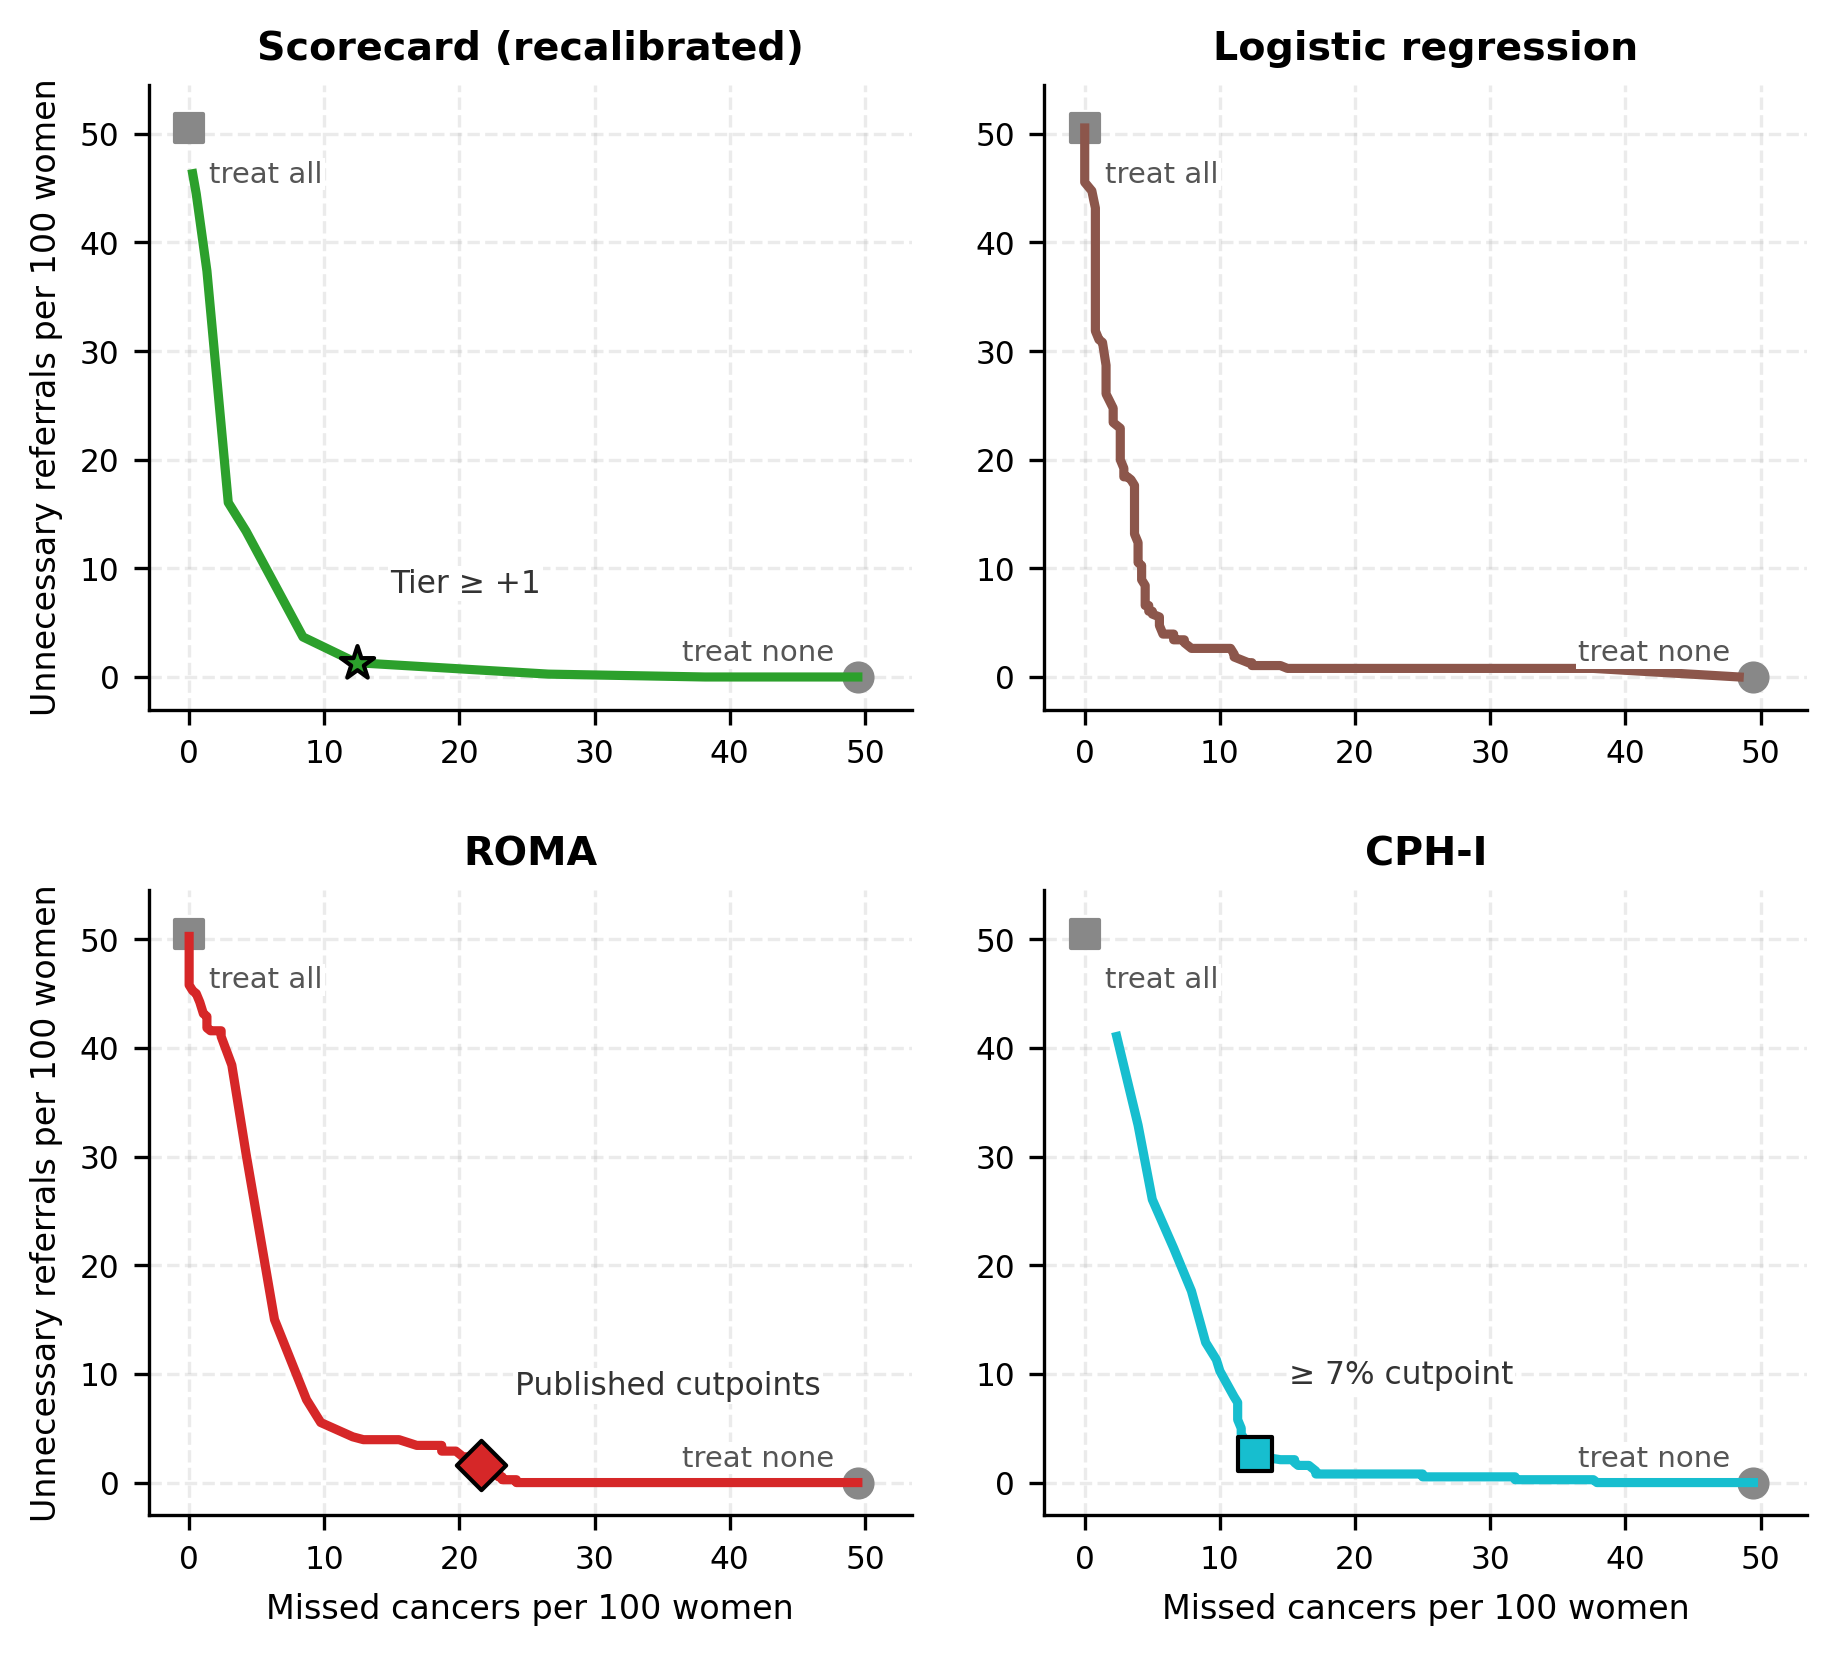
\includegraphics[width=0.40\textwidth]{figures/fig_consequences}}
\end{figure*}

\subsection{Robustness and data efficiency}

\paragraph{Measurement noise.} Under 30\% multiplicative noise on CA125/HE4
the scorecard lost 0.040 AUROC ($-4.3\%$), versus $-0.002$ for the
unbinned regression, $-0.074$ (ROMA), and $-0.086$ (XGBoost)
(\figureref{fig:noise}). The ordering was the same under additive noise,
combined noise, and 5\% gross-error contamination. Shifting the frozen
tertile cutpoints by $\pm10\%$ changed the scorecard's AUROC by at most
0.016.

\begin{figure*}[htbp]
\floatconts
  {fig:noise}
  {\caption{Change in external AUROC on the West China cohort ($n=380$)
   from 0\% to 30\% multiplicative noise on CA125/HE4. Bars are mean
   changes over 100 independent perturbations; whiskers are $\pm$1 SD
   across perturbations.}}
  {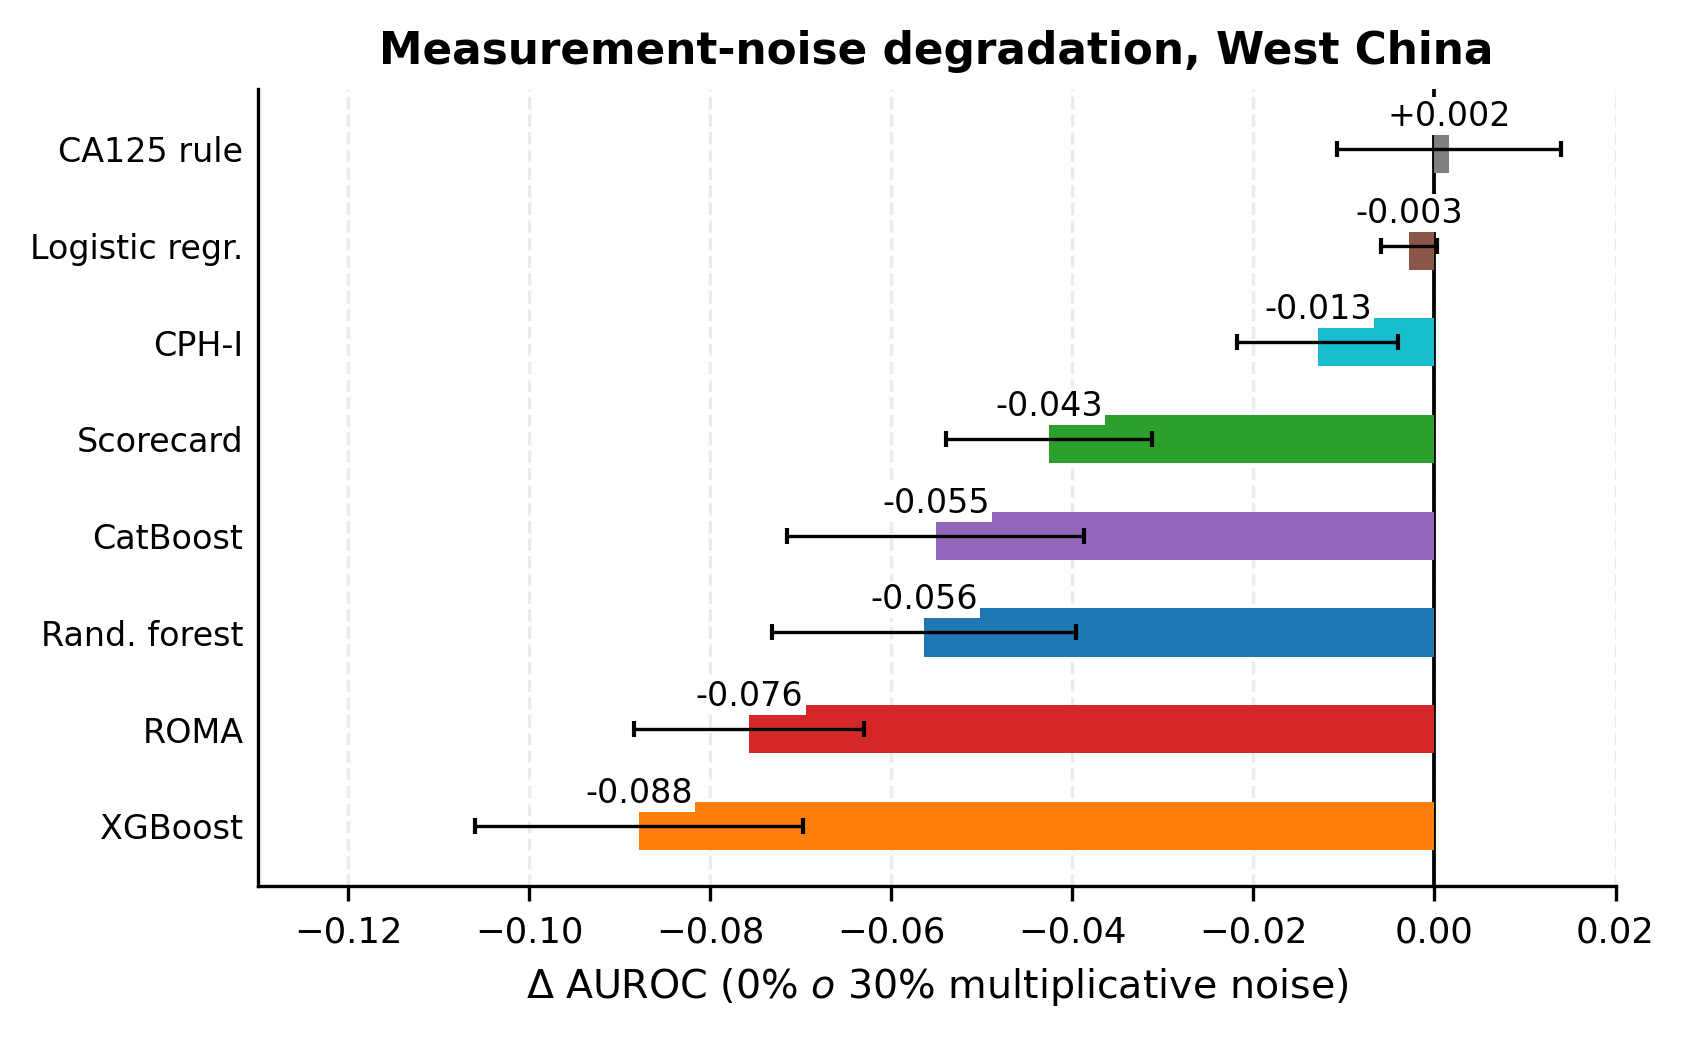
\includegraphics[width=0.66\textwidth]{figures/fig_noise}}
\end{figure*}

\paragraph{Data efficiency.} In the learning curves
(\figureref{fig:learning}), the unbinned regression reached 0.925 at
$n=60$ and 0.936 at $n=349$; the scorecard 0.901$\to$0.929; the ensembles
never exceeded 0.90 at any training size.

\begin{figure*}[htbp]
\floatconts
  {fig:learning}
  {\caption{External learning curves on West China ($n=380$), one panel
   per model: models refitted on stratified training subsamples of size
   $n \\in \\{60,90,120,180,240,349\\}$ and evaluated frozen on West China.
   Points are means $\pm$ SD over 10 draws; the dashed line marks ROMA's
   fixed-formula AUROC. Panel titles give each model's minimum-to-maximum
   external AUROC over the training sizes.}}
  {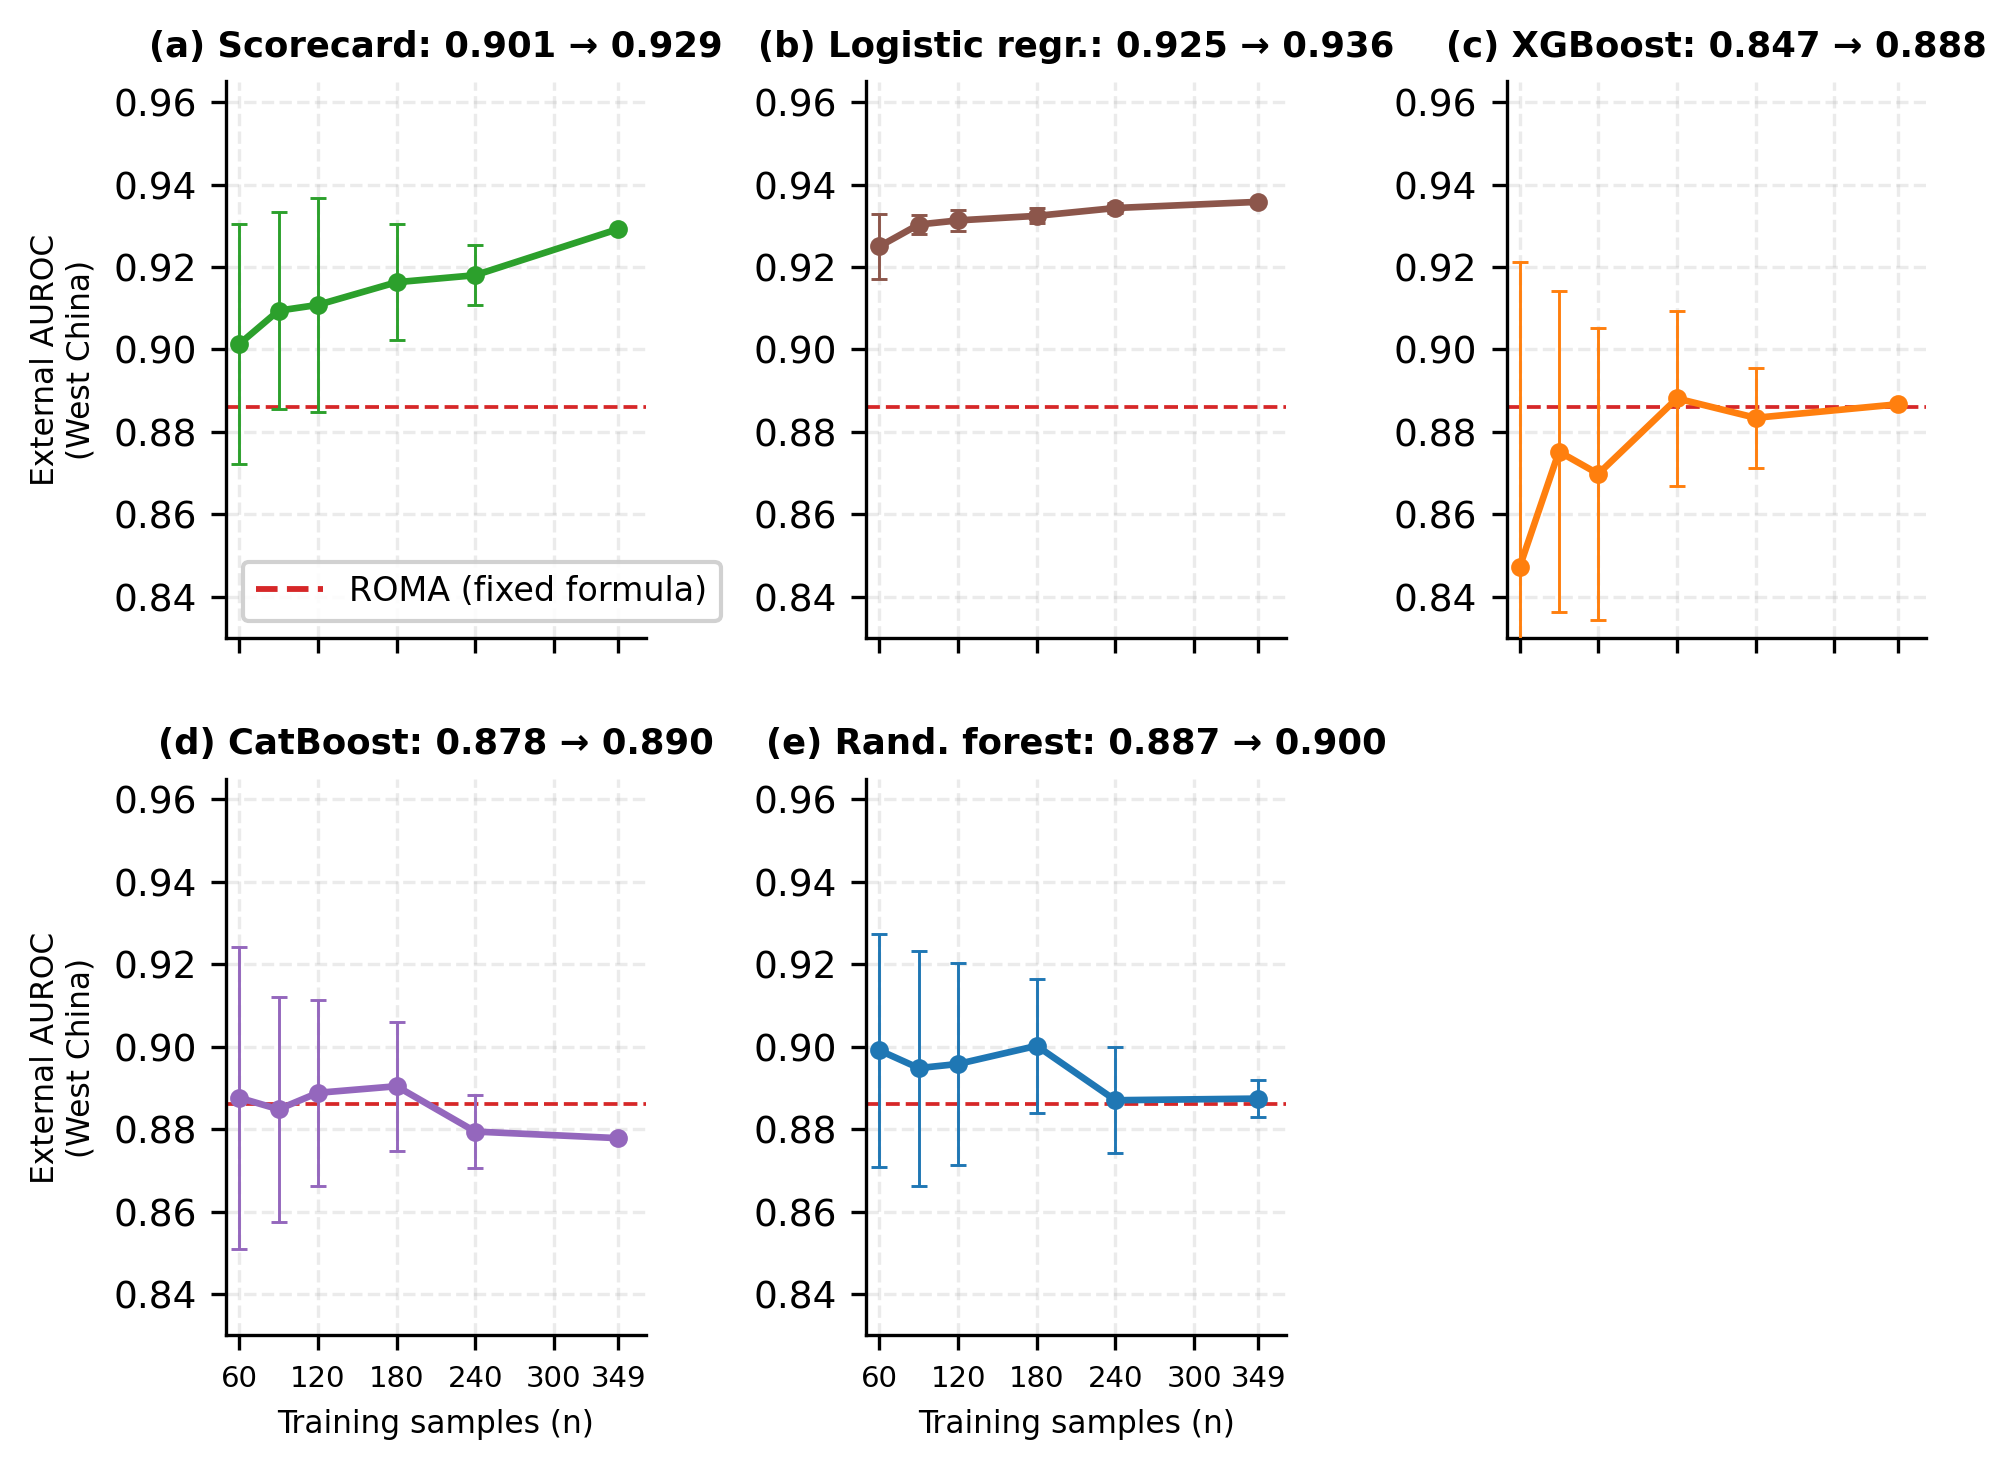
\includegraphics[width=0.58\textwidth]{figures/fig_learning}}
\end{figure*}

\paragraph{Missing-data sensitivity.} For patients whose HE4 or age was median-imputed, evaluation used the
remaining complete features. On the 100 patients with measured
HE4 (63 cancers), every model's AUROC was at least as high as on the full
cohort (\tableref{tab:completecase}). Refitting the models without
HE4 changed the scorecard's West China AUROC by 0.004 (0.925), the
unbinned regression's by 0.004 (0.932), and XGBoost's by $+0.004$ (0.891).

\begin{table}[htbp]
\floatconts
  {tab:completecase}
  {\caption{Complete-case sensitivity on West China: AUROC restricted to
   the 100 patients with measured HE4 (63 cancers), versus the full cohort
   ($n=380$; median-imputed HE4).}}
  {\setlength{\tabcolsep}{3pt}\begin{tabular}{lcc}
  \toprule
  Model & Full ($n{=}380$) & Complete ($n{=}100$)\\
  \midrule
  Scorecard & 0.929 & 0.971\\
  Logistic reg. & 0.936 & 0.978\\
  ROMA & 0.886 & 0.965\\
  XGBoost & 0.887 & 0.923\\
  \bottomrule
  \end{tabular}}
\end{table}

\subsection{Simulation}

\paragraph{Simulation.} Under stationary structure, CatBoost exceeded the
scorecard by 0.01--0.05 across cells, and the purely linear regression
trailed by 0.06--0.21. Under concept drift, the scorecard ranked first in
22 of 24 cells; the ensembles were 0.01--0.04 below it, and the unbinned
regression was within 0.02--0.07 of it (\figureref{fig:regime}). In the
factor decomposition (\tableref{tab:factors}), the gap spread across drift
levels was 0.033. The spreads were 0.003 for training size, 0.012 for
distribution shift, and 0.002 for noise. At partial drift ($d=0.5$) the
XGBoost-minus-scorecard gap was $-0.016$ (between $+0.009$ at $d=0$ and
$-0.025$ at $d=1$); the CatBoost gap was $+0.024$, $+0.006$, and $-0.006$
at $d=0,0.5,1$. The empirical cohorts had mean KS shifts of
0.22--0.50 relative to training.

\begin{table}[htbp]
\floatconts
  {tab:factors}
  {\caption{Factor decomposition of the XGBoost-minus-scorecard test AUROC
   gap in the simulation (factor levels: drift 0/1, shift 0--1, size
   100--800, noise 0/0.5). The spread across drift levels (0.033) was
   larger than across any other factor (0.002--0.012). Under stationary
   structure CatBoost won all 24 cells; under drift the scorecard won 22
   of 24.}}
  {\small\begin{tabular}{lcc}
  \toprule
  Factor & Gap range & Spread\\
  \midrule
  Concept drift & $+0.007$ $\to$ $-0.026$ & \textbf{0.033}\\
  Distribution shift & $-0.015$ $\to$ $-0.003$ & 0.012\\
  Training size & $-0.011$ $\to$ $-0.008$ & 0.003\\
  Measurement noise & $-0.010$ $\to$ $-0.009$ & 0.002\\
  \bottomrule
  \end{tabular}}
\end{table}

\begin{figure*}[htbp]
\floatconts
  {fig:regime}
  {\caption{Regime map from the synthetic study: cell values are mean
   XGBoost-minus-scorecard test AUROC across 20 replicates per cell (50\%
   measurement noise), by training size and distribution shift.
   (a) Stationary structure. (b) Concept drift.}}
  {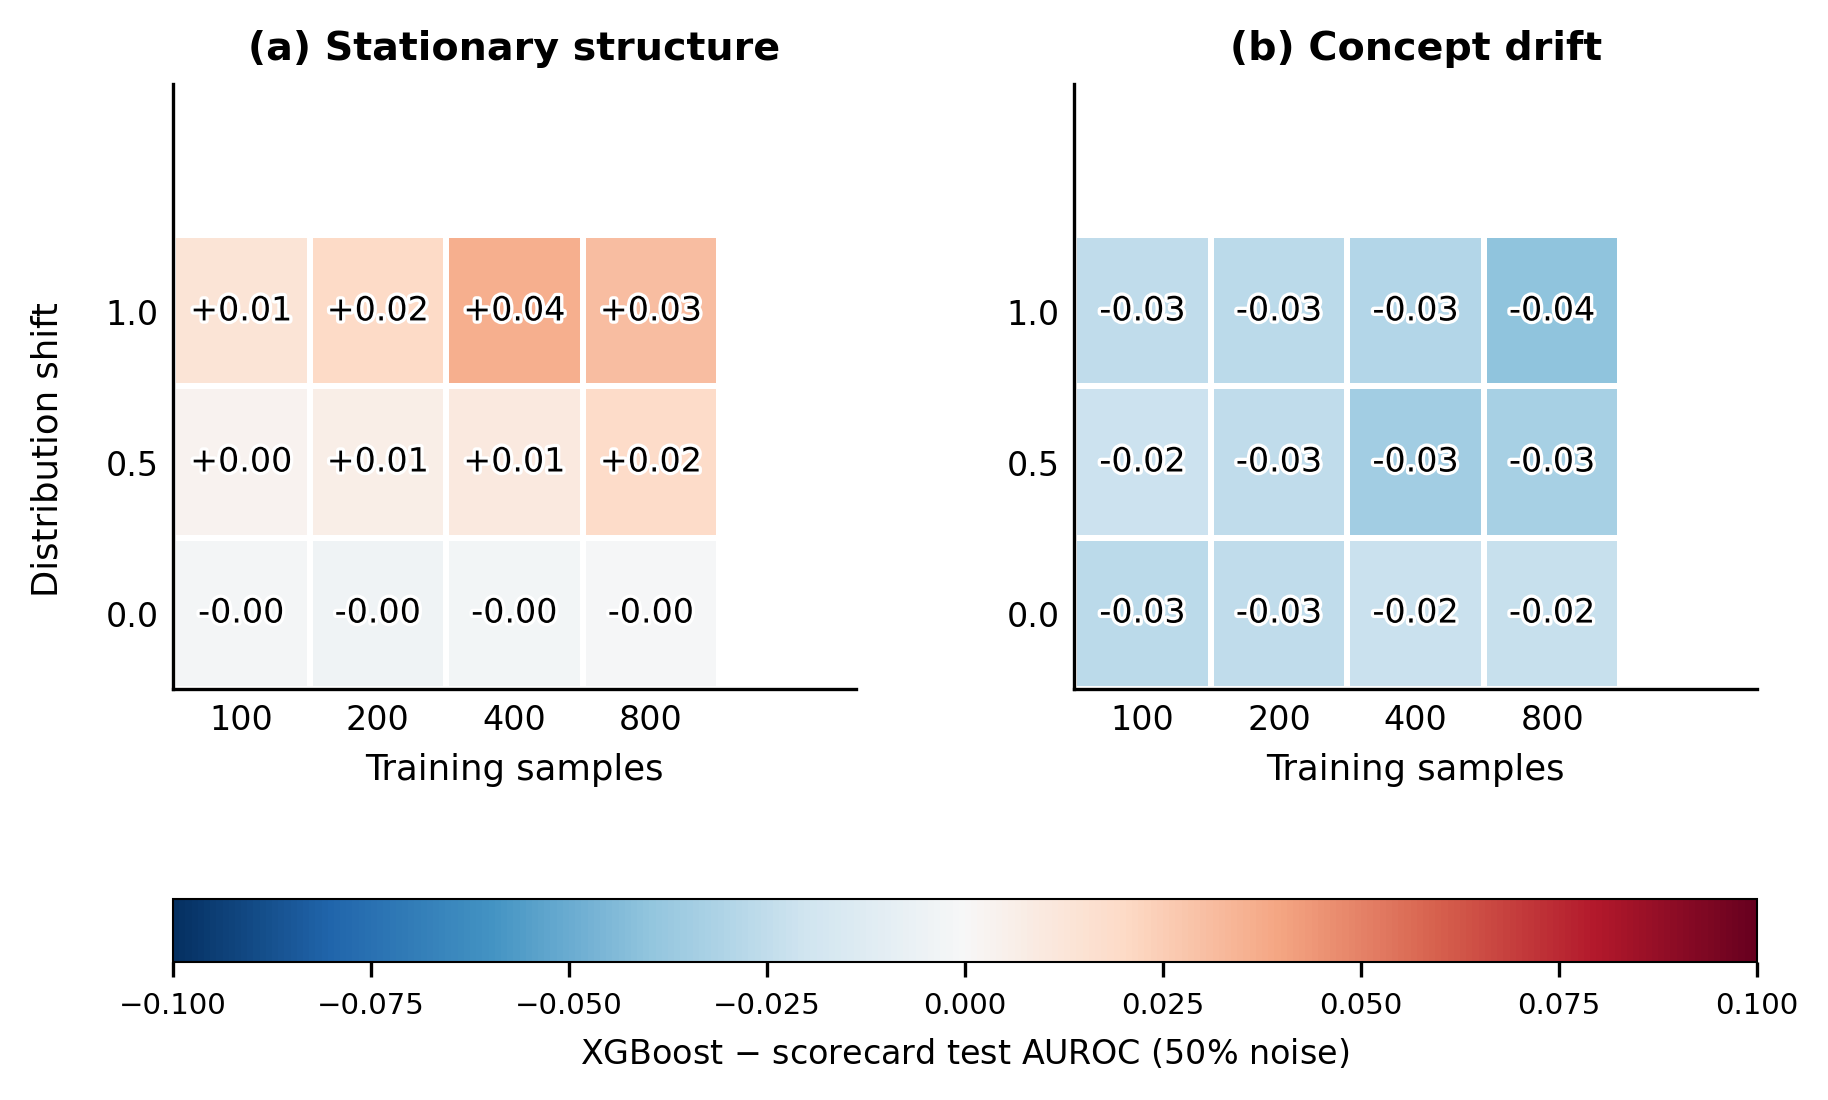
\includegraphics[width=0.60\textwidth]{figures/fig_regime}}
\end{figure*}

\subsection{Reclassification and sensitivity analyses}

\paragraph{Reclassification.} The integrated discrimination improvement of the scorecard's frozen map
was $+0.071$ (95\% CI 0.036--0.106) versus ROMA, $+0.110$ versus CPH-I,
$-0.048$ versus the unbinned regression, and $-0.197$ versus XGBoost; the
category-free NRI versus ROMA was $-0.23$ (event $+0.68$, non-event
$-0.91$) \citep{pencina2008}.

\paragraph{Sensitivity analyses.} Across the 12 L2 selection candidates, five-fold CV ranged
0.900--0.913. The configuration maximizing internal CV (4 bins, CV 0.913)
achieved 0.880 externally; the selected three-bin configuration (CV 0.907)
achieved 0.929. L1 variants reached 0.907
externally and two-bin configurations 0.847. The tuned tree ensembles (best
of 27 configurations per family) reached 0.890 (XGBoost), 0.877
(CatBoost), and 0.894 (Random Forest) on
West China. A training-fitted KNN imputation of the Japanese missing
values (outcome-correlated) gave 0.907; the frozen-median convention was
retained.

\section{Discussion and Limitations}

Three findings stand out. First, at $n<400$ the discrimination ceiling
is reachable with seven integer parameters; further degrees of freedom
\emph{cost} external performance, extending \citep{christodoulou2019}.
Second, the published cutpoints missed 82 of 188 cancers at a prevalence
(49.5\%) far from the Western development prevalence---base-rate
dependence \citep{rolfsen2020}---and a locally calibrated scorecard
dominates them at all rates $\le10{:}1$. Third, the simulation offers a
plausible mechanistic account in which \emph{concept drift} produces the
observed ranking; the factor decomposition and nonlinearity-strength sweep
show it is graded rather than an artifact, and it is a falsifiable probe
rather than a demonstration that drift occurred.
For deployment, the chosen model class determines how a tool behaves
when population and assay platform change---a failure mode internal
evaluation cannot reveal. The protocol---frozen external cohorts, meta-analytic pooling, decision
consequences, a drift-aware simulation---is proposed as a default template
for small-sample clinical ML \citep{collins2015}.

\emph{Scope.} The benchmark is serum-only because the public cohorts lack
imaging variables; ultrasound-based models (RMI, IOTA ADNEX) are the
standard of care where imaging is available, and no superiority over them
is claimed. Findings apply to serum-based triage, where ultrasound is
unavailable or a first-stage screen.

Limitations: the external cohorts exhibit observed distribution shift
(per-feature KS statistics 0.22--0.50 relative to training), whereas
concept drift is a property of the simulation---it is not directly measured
in the real data, and the simulation's role is to show that drift
\emph{can} produce the observed ranking, not that it did. The Japanese
stress-test cohort has 27 cancers ($\sim$20\% power for a 0.05 difference);
because its controls are healthy women, its specificity estimates are not
interpretable as triage specificities; it is used only to bound
discrimination under case-mix shift. Single geographic region; prospective
validation pending.

\bibliography{ref}

\appendix

\section{Supplementary Details}

\paragraph{Deployed scorecard.} Integer weights
(CA125/HE4/age/menopause): bins $[-1,0,+2]$ / $[-4,-1,+5]$ / $[-2,0,+2]$ /
$[0,0,0]$; score range $-7$ to $+9$. Tertile cutpoints in training units:
CA125 24.3/165.0 U/mL, HE4 45.8/92.7 pmol/L, age 37.0/52.0 years.

\paragraph{Nonlinearity-strength sweep.} We test whether the regime map
depends on the hand-crafted outcome model by repeating the sweep at four
strengths $\gamma\in\{0.4,0.8,1.6,2.4\}$ of the injected
interaction/sinusoidal terms of \equationref{eq:eta} ($n=200$, 50\% noise,
20 replicates). The
mechanism is graded rather than knife-edge: the ensembles'
stationary-regime advantage grows monotonically with $\gamma$ (CatBoost
$+0.01$ to $+0.05$), and under drift it erodes monotonically, crossing to a
scorecard advantage of $-0.01$ to $-0.04$ once $\gamma\ge1.6$; at
$\gamma\le0.8$ no class has an appreciable edge in either regime. The
conclusion requires only learnable nonlinear structure that drifts, not a
specific generative model. Ensemble-minus-scorecard gaps (mean over shift
cells):

\begin{table}[h]
\floatconts
  {tab:gammasweep}
  {\caption{Ensemble-minus-scorecard gaps across nonlinearity strengths.}}
  {\small\begin{tabular}{lcccc}
  \toprule
  & \multicolumn{2}{c}{CatBoost $-$ scorecard} & \multicolumn{2}{c}{XGBoost $-$ scorecard}\\
  $\gamma$ & Stationary & Drift & Stationary & Drift\\
  \midrule
  0.4 & $+0.007$ & $+0.005$ & $-0.013$ & $-0.017$\\
  0.8 & $+0.008$ & $+0.007$ & $-0.008$ & $-0.013$\\
  1.6 & $+0.028$ & $-0.006$ & $+0.014$ & $-0.026$\\
  2.4 & $+0.050$ & $-0.017$ & $+0.038$ & $-0.035$\\
  \bottomrule
  \end{tabular}}
\end{table}

\end{document}
